\section{Pathway Browser Implementation}
\label{sect:maw_implementation}

\mawapp must track a few different categories of data. The most basic is a
representation of the data model of the online PathCase MAW database, derived
from the web service interface to the database. Examples include pathways,
metabolites, compartments, and processes. In Model-View-Controller terms (see
\ref{sect:cocoa_mvc}), these are \emph{model} classes.  These model
objects are rendered in \emph{views}, such as the main pathway graph view.
The models and views are managed by \emph{controllers} which manipulate the
models and configure the views.

Section \ref{sect:smda_arch_overview} describes the general architecture of
\mawapp. Section \ref{sect:smda_data_model} describes the subset of the
\pathcasemaw data model that is used by \mawapp. Section
\ref{sect:smda_web_services_server} enumerates the web services that
\pathcasemaw provides to download these model objects into \mawapp. Section
\ref{sect:smda_web_services_client} explains how \mawapp accesses these web
services and converts their results into model objects to be used by the
application. Finally, section \ref{sect:smda_rendering} describes how the model
objects are rendered to the screen.

\subsection{Architecture Overview}
\label{sect:smda_arch_overview}

\begin{figure}[p]
    \center{
        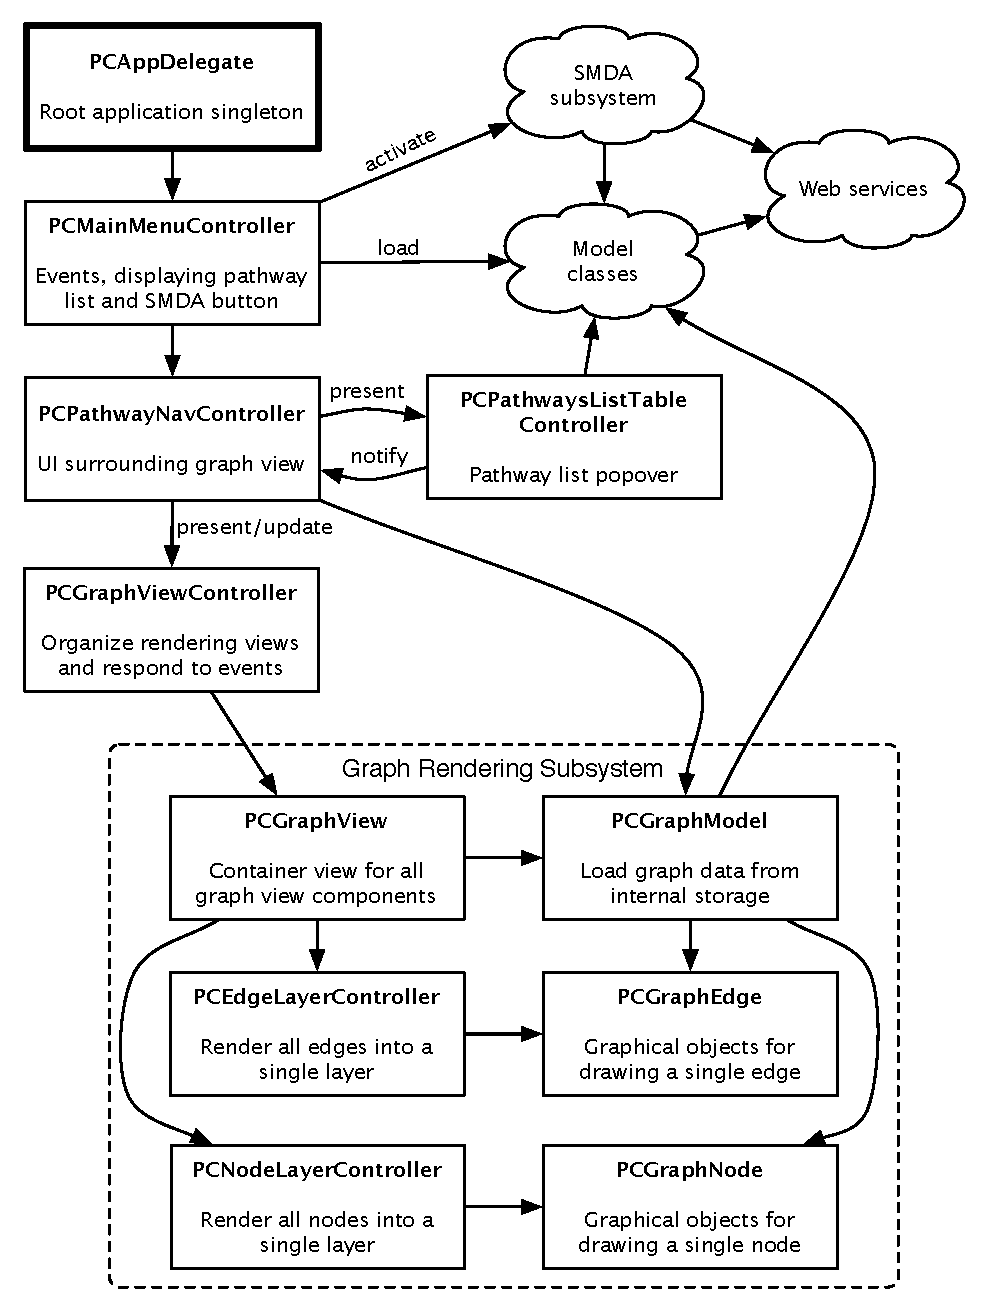
\includegraphics[width=\textwidth]{maw/figures/components.pdf}}
    \caption{\label{fig:maw_components} Components of the architecture. See
    \ref{sect:smda_arch_overview} for more information about this diagram.}
\end{figure}

Figure \ref{fig:maw_components} shows a high-level representation of the
relationships between the most important objects in \mawapp.

An application-level singleton, \texttt{PCAppDelegate}, handles
application-level delegate methods and notifications from the system. Another
singleton, \texttt{PCMainMenuViewController}, displays the home screen,
including the list of pathways and button to enter SMDA. It also initiates the
download of the model objects if they require an update. This relationship is
represented by the \emph{activates} and \emph{loads} arrows in figure
\ref{fig:maw_components}.

When an item in the list of pathways is tapped, a new view is shown, controlled
by \texttt{PCPathwayNavController}. This view controller object controls the
toolbar and a content area that can contain any view and corresponding view
controller. See the screenshot in figure \ref{fig:maw_screenshot_pathway} to see
how this toolbar is displayed to the user.

The content area is controlled by \texttt{PCGraphViewController}. This view
controller object controls a \texttt{PCGraphView} which renders the pathway
visualization based on a \texttt{PCGraphModel} and sends notifications back to
the \texttt{PCGraphViewController} if an event occurs (e.g. a node being tapped).

As shown in figure \ref{fig:maw_screenshot_pathway_list_popover}, the
``Pathways'' button in the toolbar controlled by \texttt{PCPathwayNavController}
displays a list of pathways that may be visualized. The loading and display of
this list is handled by \texttt{PCPathwayListTableController}, which loads
pathway model objects (\ref{sect:smda_data_model}) and converts them
to a list to be displayed by a table view (\ref{sect:ipad_views}). When a table
view row is selected, the \texttt{PCPathwayListTableController} sends a
notification back to the \texttt{PCPathwayNavController}, which replaces its
content area with a \texttt{PCGraphViewController} representing the new pathway
to be displayed.

The control flow of \texttt{PCPathwayNavController} at runtime is shown in
figure \ref{fig:maw_controlflow}. This object has no event loop of its own; its
functionality is invoked by the application event loop provided by the Cocoa
framework. When the ``Pathways'' button is pressed, it creates a
\texttt{PCPathwayListTableController} which presents a popover containing a
table view, loads the list of pathways, populates the table view, and sends
control back to the event loop. When a row is tapped in this table view, the
\texttt{PCPathwayListTableController} sends a notification back to the
\texttt{PCPathwayNavController}, which hides the popover, loads the new pathway
visualization, and displays it.

\begin{figure}[thbp]
    \center{
        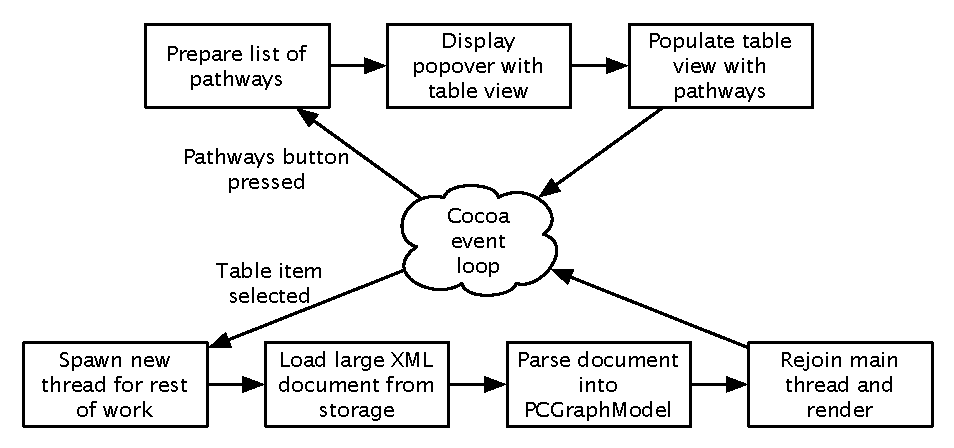
\includegraphics[width=5in]{maw/figures/controlflow.pdf}}
    \caption{\label{fig:maw_controlflow} Control flow of
    \texttt{PCPathwayNavController}}
\end{figure}

\texttt{PCGraphViewController} and \texttt{PCGraphModel} are the high level
interface to the pathway visualization subsystem. \texttt{PCGraphModel} holds
collections (hash tables) of \texttt{PCGraphNode} and \texttt{PCGraphEdge}
objects. These objects represent the visual properties of each node and edge in
the graph, including location, color, shape, label text, and label position. The
\texttt{PCGraphViewController} and its helper objects render the graph
represented by the \texttt{PCGraphModel} to a scroll view
that the user can navigate by touch (\ref{sect:ipad_views}). 

\subsection{Data Model}
\label{sect:smda_data_model}



\subsection{Web Services: Server Side}
\label{sect:smda_web_services_server}

\subsection{Web Services: Client Side}
\label{sect:smda_web_services_client}

Although the data is accessed via web services, it is needed so often and is
small enough that the entire database is distributed with the application
package in the form of serialized objects. The database can be updated whenever
the user chooses via the user interface.

Each web service corresponds roughly to one data type in the model, so those
model objects contain methods to load their data from the corresponding web
service. For example, the method \texttt{[PCPathway loadDataFromServer]}
updates all pathway objects. However, this method relies on some data for
tissues and metabolites to have been downloaded already, so the data update
process uses mutexes and asynchronous network requests to ensure that the data
is downloaded in the correct order while using parallelism as much as possible.

These web service fetching methods convert the XML response of the web service
into corresponding model objects (such as \texttt{SMDAPathway}) which are
serialized to the device's internal storage.

\begin{figure}[thbp]
    \center{
        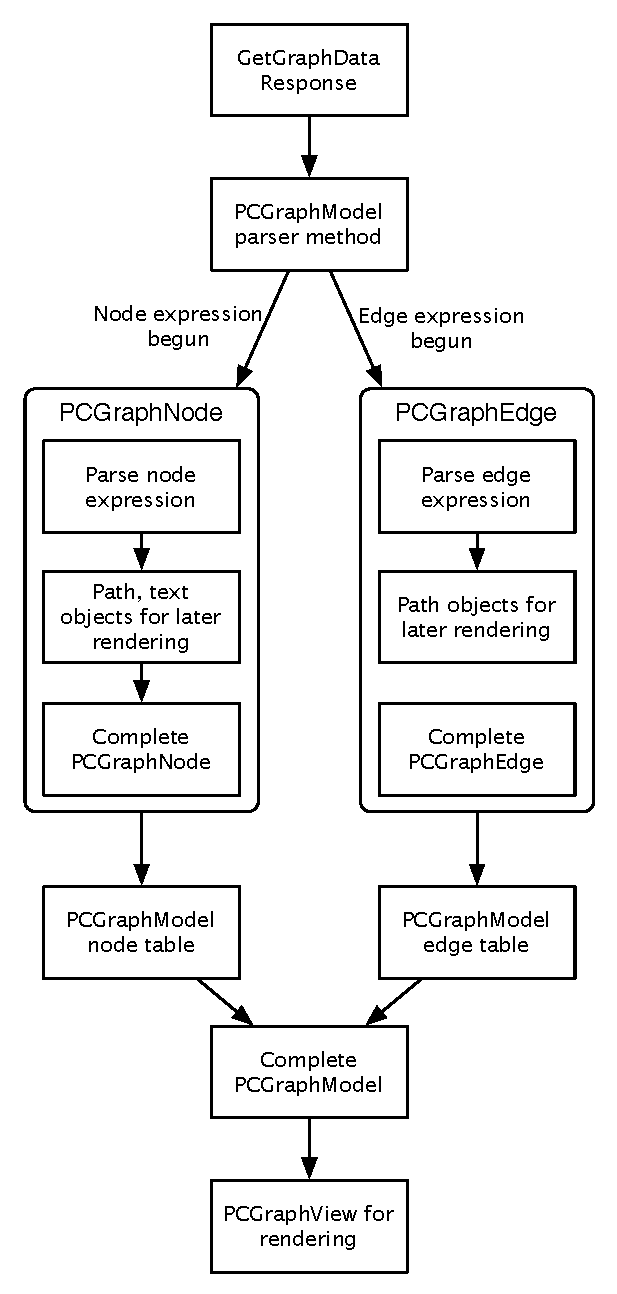
\includegraphics[width=4in]{maw/figures/dataflow.pdf}}
    \caption{\label{fig:maw_dataflow} Data flow for graph data}
\end{figure}

\subsection{Rendering}
\label{sect:smda_rendering}
